%!TEX program = xelatex
\documentclass[cn,blue,normal,founder,11pt]{elegantnote}

\hypersetup{
			pdftitle={图论三次作业},
			pdfauthor={李徐瑾}
}

\usepackage{amssymb}
\usepackage{mathtools}
\usepackage{float}
\let\Bbbk\undefined
\usepackage[complete,subscriptcorrection,slantedGreek]{mtpro2}
\let\qedhere\undefined
\newcommand{\calO}{\mathcal{O}}
\newcommand{\bbN}{\mathbb{N}}
\renewcommand{\qed}{\(\hfill\square\)}
\renewcommand{\proofname}{\normalfont\bfseries\color{ecolor}解}


\title{图论第三次作业}
\institute{数学科学学院}
\author{李徐瑾\quad 202021110109}
\date{\zhtoday}

\begin{document}

\maketitle

\centerline{\includegraphics[scale=0.16]{image/UESTC_cp.pdf}}
\section{习题六}

\begin{example}
	设\(G\)是一个有\(n\)个点\(m\)条边的简单连通平面图,则
	\begin{enumerate}[(1)]
		\item 若每个面至少由四条边围成,则\(m\leqslant 2n-4\);
		\item 若每个面至少由五条边围成,则\(3m\leqslant 5n-10\);
		\item 若每个面至少由六条边围成,则\(2m\leqslant 3n-6\).
	\end{enumerate}
\end{example}

\begin{proof}
设图\(G\)有\(\phi\)个面且面最小的次数为\(l\),根据次数公式,则有
\[2m=\sum_{\phi\in\Phi(G)}\phi\deg(\phi)\geqslant l\phi.\]
结合欧拉公式\(n-m+\phi=2\),则有
\[m\leqslant\frac{l}{l-2}(n-2).\]
\begin{enumerate}[(1)]
	\item 此时\(l\geqslant 4\),故\(m\leqslant 2n-4\);
	\item 此时\(l\geqslant 5\),故\(3m\leqslant 5n-10\);
	\item 此时\(l\geqslant 6\),故\(2m\leqslant 3n-6\).  
\end{enumerate}
\end{proof}

\begin{example}
	设\(G\)是有\(n(n\geqslant 3)\)个点\(\phi\)个面的简单连通平面图. 证明: \(\phi\leqslant 2n-4\).
\end{example}

\begin{proof}
	设图\(G\)有\(m\)条边且每个面的次数满足\(l\geqslant 3\),根据次数公式,则有
	\[2m=\sum_{\phi\in\Phi(G)}\phi\deg(\phi)\geqslant 3\phi.\]
	结合欧拉公式\(n-m+\phi=2\),则有
	\begin{align*}
		\phi&=2-n+m\\
		&\geqslant 2-n+3\phi/2\\
		&\Rightarrow\phi\leqslant 2n-4.
	\end{align*}
\end{proof}

\begin{example}
	设\(G\)是一个有\(n(n\geqslant 3)\)个点\(m\)条边\(\phi\)个面的极大平面图,则
	\begin{enumerate}[(1)]
		\item \(m=3n-6\);
		\item \(\phi=2n-4\);
		\item \(\kappa(G)\geqslant 3\).
	\end{enumerate}
\end{example}

\begin{proof}
	\begin{enumerate}
		\item[(1-2)] 图\(G\)的每个面的次数均为\(3\). 根据次数公式,则有
		\[2m=3\phi.\] 
		结合欧拉公式\(n-m+\phi=2\),则有
		\begin{align*}
			m&=3n-6,\\
			\phi&=2n-4.
		\end{align*}
		\item[(3)] 图\(G\)是\(2\)连通的. 当\(n=4\)时,\(G=K_4\),命题成立. 采用数学归纳法. 设\(n<k(k\geqslant 5)\)时命题成立. 现置\(n=k,\kappa(G)=2\). 则存在\(V\)的子集\(V_1,V_2\)满足\(V_1\cup V_2\subset V\)使得
		\[G_1=G[V_1],\quad G_2=G[V_2],\quad G_1\cap G_2=\{uv\}.\]
		我们断定\(uv\in E(G)\). 若不然,由于图\(G\)是极大平面图,则\(G+uv\)不可平面. 根据Kuratowski定理,\(G+uv\)包含了\(K_5\)或\(K_{3,3}\)的同胚子图,故\(uv\in E(G)\). 易知\(G_1\)和\(G_2\)均是极大平面图,因此\(G_1\)和\(G_2\)在三角形和\(3\)连通中两者必居其一. 事实上,我们可选取一种平面嵌入使得\(uv\)是\(G_1\)和\(G_2\)的边界,且存在\(w_1\in V(G_1),w_2\in V(G_2)\)分别在边界面上,此时\(G+w_1w_2\)是可平面的,矛盾.
	\end{enumerate}
\end{proof}

\begin{example}
	试证: 没有\(6\)连通的可平面图.
\end{example}

\begin{proof}
	反证法. 假设图\(G\)是\(6\)连通的可平面图,则有\(\kappa(G)\geqslant 6\). 已知
	\[\kappa(G)\leqslant\lambda(G)\leqslant\delta(G),\]
	因此\(\delta(G)\geqslant 6\). 根据握手定理可知
	\[2m=\sum_{v\in V(G)}d(v)\geqslant n\delta(G)=6n,\]
	即\(m\geqslant 3n>3n-6\),矛盾.
\end{proof}

\begin{example}
	试证: 若\(G\)是连通平面图,且所有顶点的度数不小于\(3\),则\(G\)至少有一个面\(f\),使得\(\deg(f)\leqslant 5\).
\end{example}

\begin{proof}
	反证法. 假设图\(G\)的每个面的次数均有\(\deg(f)\geqslant 6\). 根据次数公式,则有
	\[2m=\sum_{f\in \Phi(G)}f\deg(f)\geqslant 6f\]
	且由于图\(G\)的所有顶点的度数不小于\(3\),根据握手定理可知
	\[2m=\sum_{v\in V(G)}d(v)\geqslant n\delta(G)=3n.\]
	结合欧拉公式\(n-m+f=2\),则有
	\begin{align*}
		2&=n-m+f\\
		&\leqslant 2m/3-m+m/3\\
		&=0,
	\end{align*}
	矛盾.
\end{proof}

\begin{example}
		求图\ref{fig:6.1}中所示图的对偶图.
		\begin{figure}[H]
			\centering
			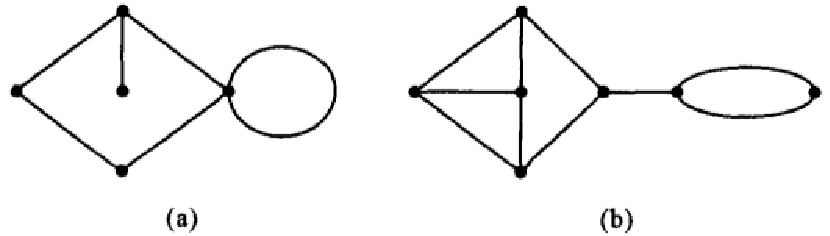
\includegraphics[scale=0.775]{image/ex20.pdf}
			\caption{}
			\label{fig:6.1}
		\end{figure}
\end{example}

\begin{proof}
	图\ref{fig:6.1}的对偶图如图\ref{fig:6.1_jie}所示.
	\begin{figure}[H]
		\centering
		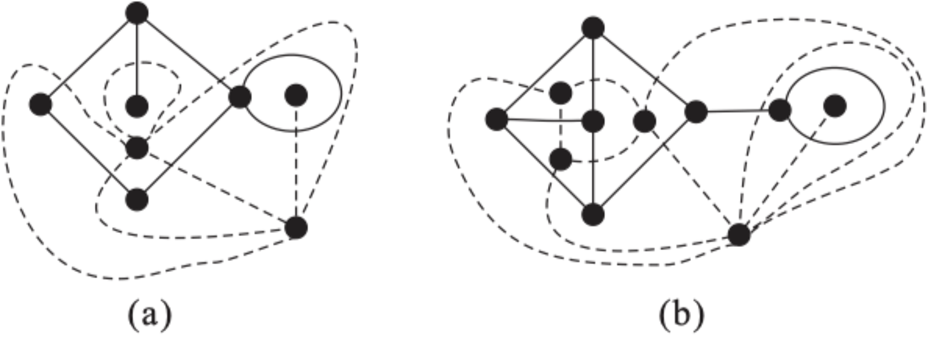
\includegraphics[scale=0.65]{image/ex20_jie.pdf}
		\caption{}
		\label{fig:6.1_jie}
	\end{figure}
\end{proof}

\section{习题七}

\begin{example}
	求图\ref{fig:7.1}各图的边色数\(\chi^{\prime}\)和色数\(\chi\),并分别给出各图的一个\(\chi^{\prime}\)边着色和\(\chi\)着色.
	\begin{figure}[H]
		\centering
		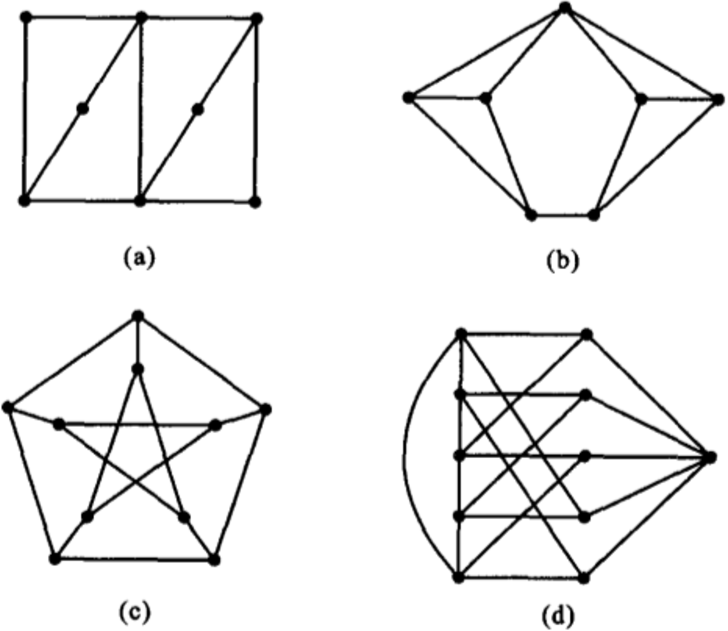
\includegraphics[scale=0.55]{image/ex7.1.pdf}
		\caption{}
		\label{fig:7.1}
	\end{figure}
\end{example}

\begin{proof}
\begin{enumerate}[(a)]
	\item 由于图\(G_a\)有两个相邻的最大度点且最大度\(\Delta=4\),故\(\chi^{\prime}(G_a)=4\);由于图\(G_a\)有顶点邻接\(2\)个顶点且邻接的顶点之间不邻接,则点色数\(\chi(G_a)\)至少为\(2\),且\(2\)种颜色能正常点着色,故\(\chi(G_a)=2\).
	\item 由于图\(G_b\)有一个最大度点且最大度\(\Delta=4\),故\(\chi^{\prime}(G_b)=4\);由于图\(G_b\)采用\(3\)着色时,不能正常点着色,但采用\(4\)着色时能正常点着色,故\(\chi(G_b)=4\).
	\item 图\(G_c\)是Peterson图,故边色数\(\chi^{\prime}(G_c)=4\),点色数\(\chi(G_c)=3\).
	\item 由于图\(G_d\)的最大度\(\Delta=5\),因此图\(G_d\)至少需要\(5\)种颜色才能正常边着色,且采用\(5\)着色时能正常边着色,故\(\chi^{\prime}(G_d)=5\);由于图\(G_d\)有顶点邻接\(4\)个顶点且邻接的顶点之间不邻接,则点色数\(\chi(G_d)\)至少为\(2\),而\(2\)种颜色不能正常点着色,但采用\(3\)着色时能正常点着色,故\(\chi(G_d)=3\).
\end{enumerate}
图\ref{fig:7.1}各图的一个\(\chi^{\prime}\)边着色和\(\chi\)着色分别如图\ref{fig:7.1edge}和图\ref{fig:7.1dot}所示.
\begin{figure}[H]
	\centering
	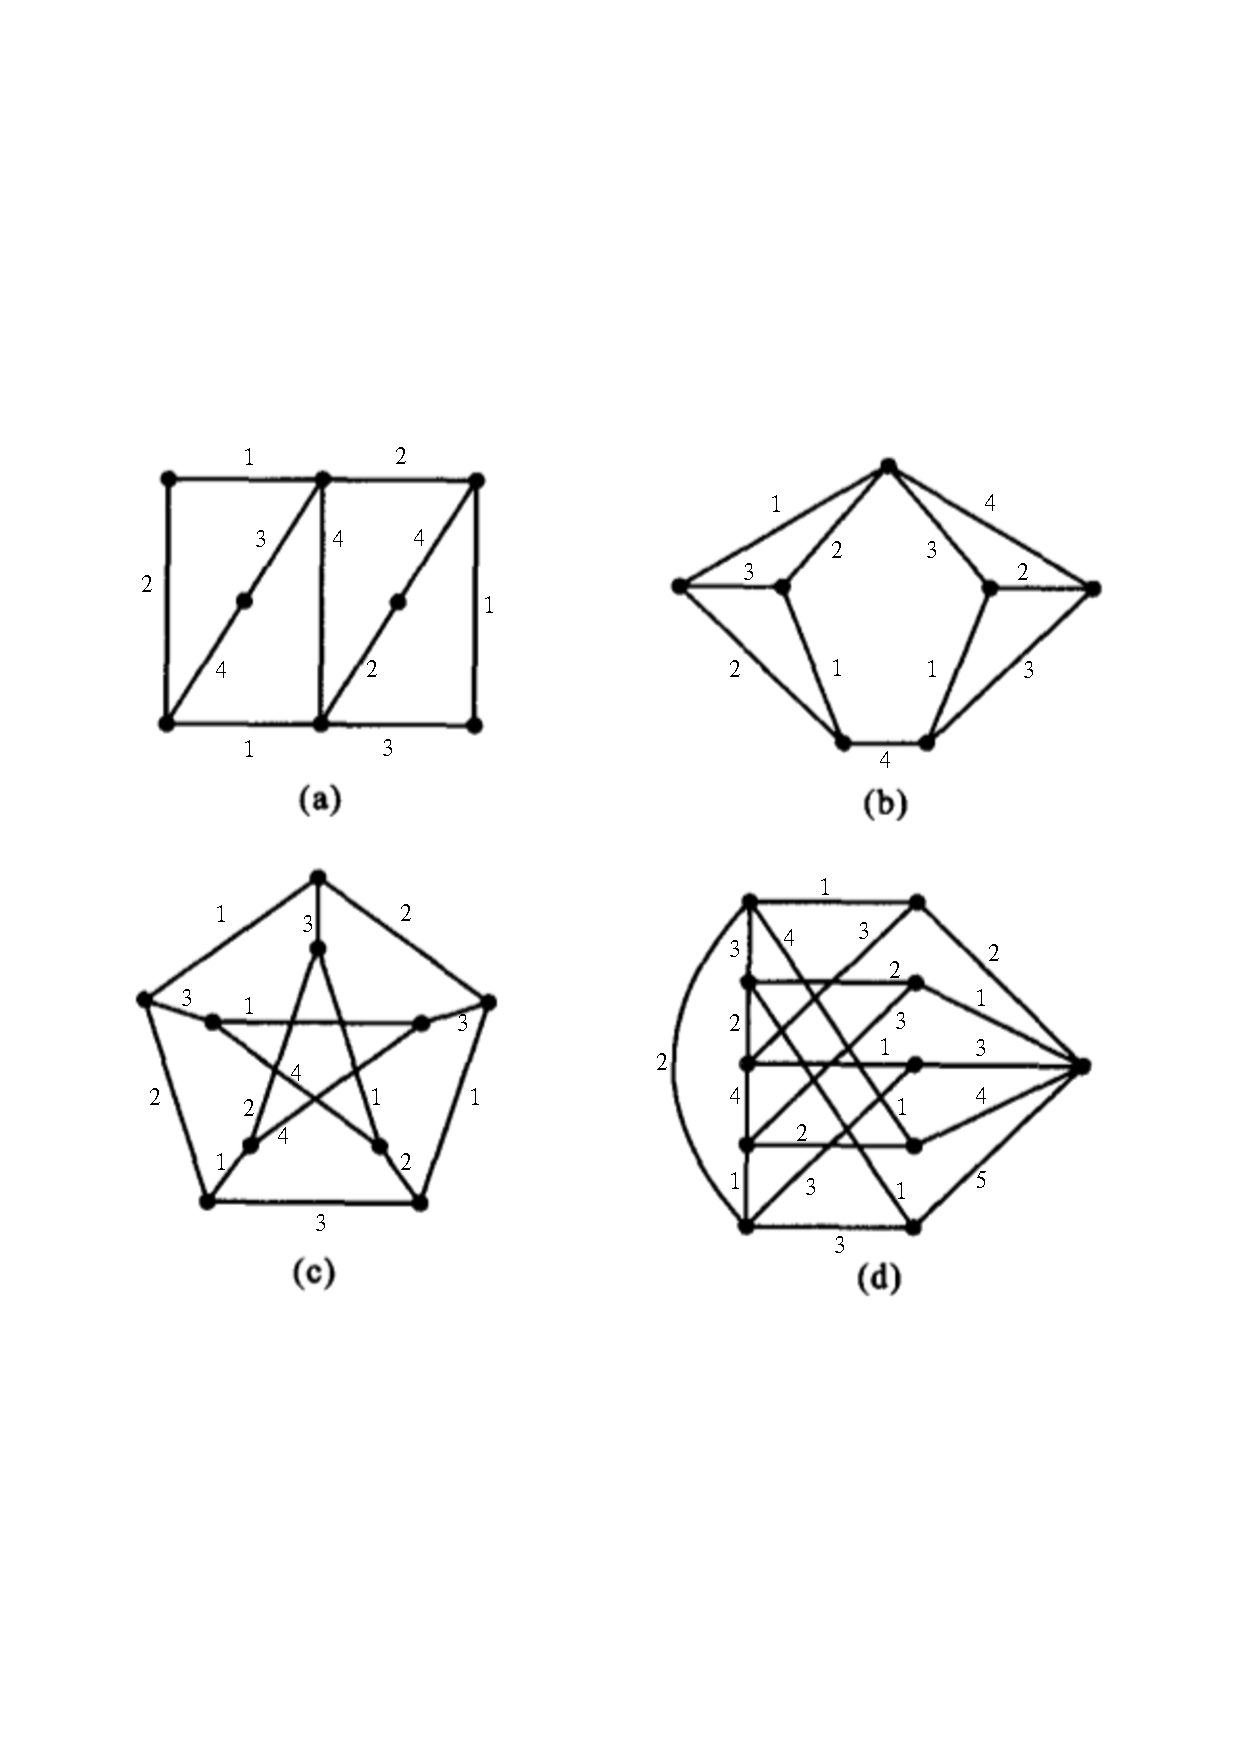
\includegraphics[scale=0.45]{image/ex7.1edge.pdf}
	\caption{}
	\label{fig:7.1edge}
\end{figure}
\begin{figure}[H]
	\centering
	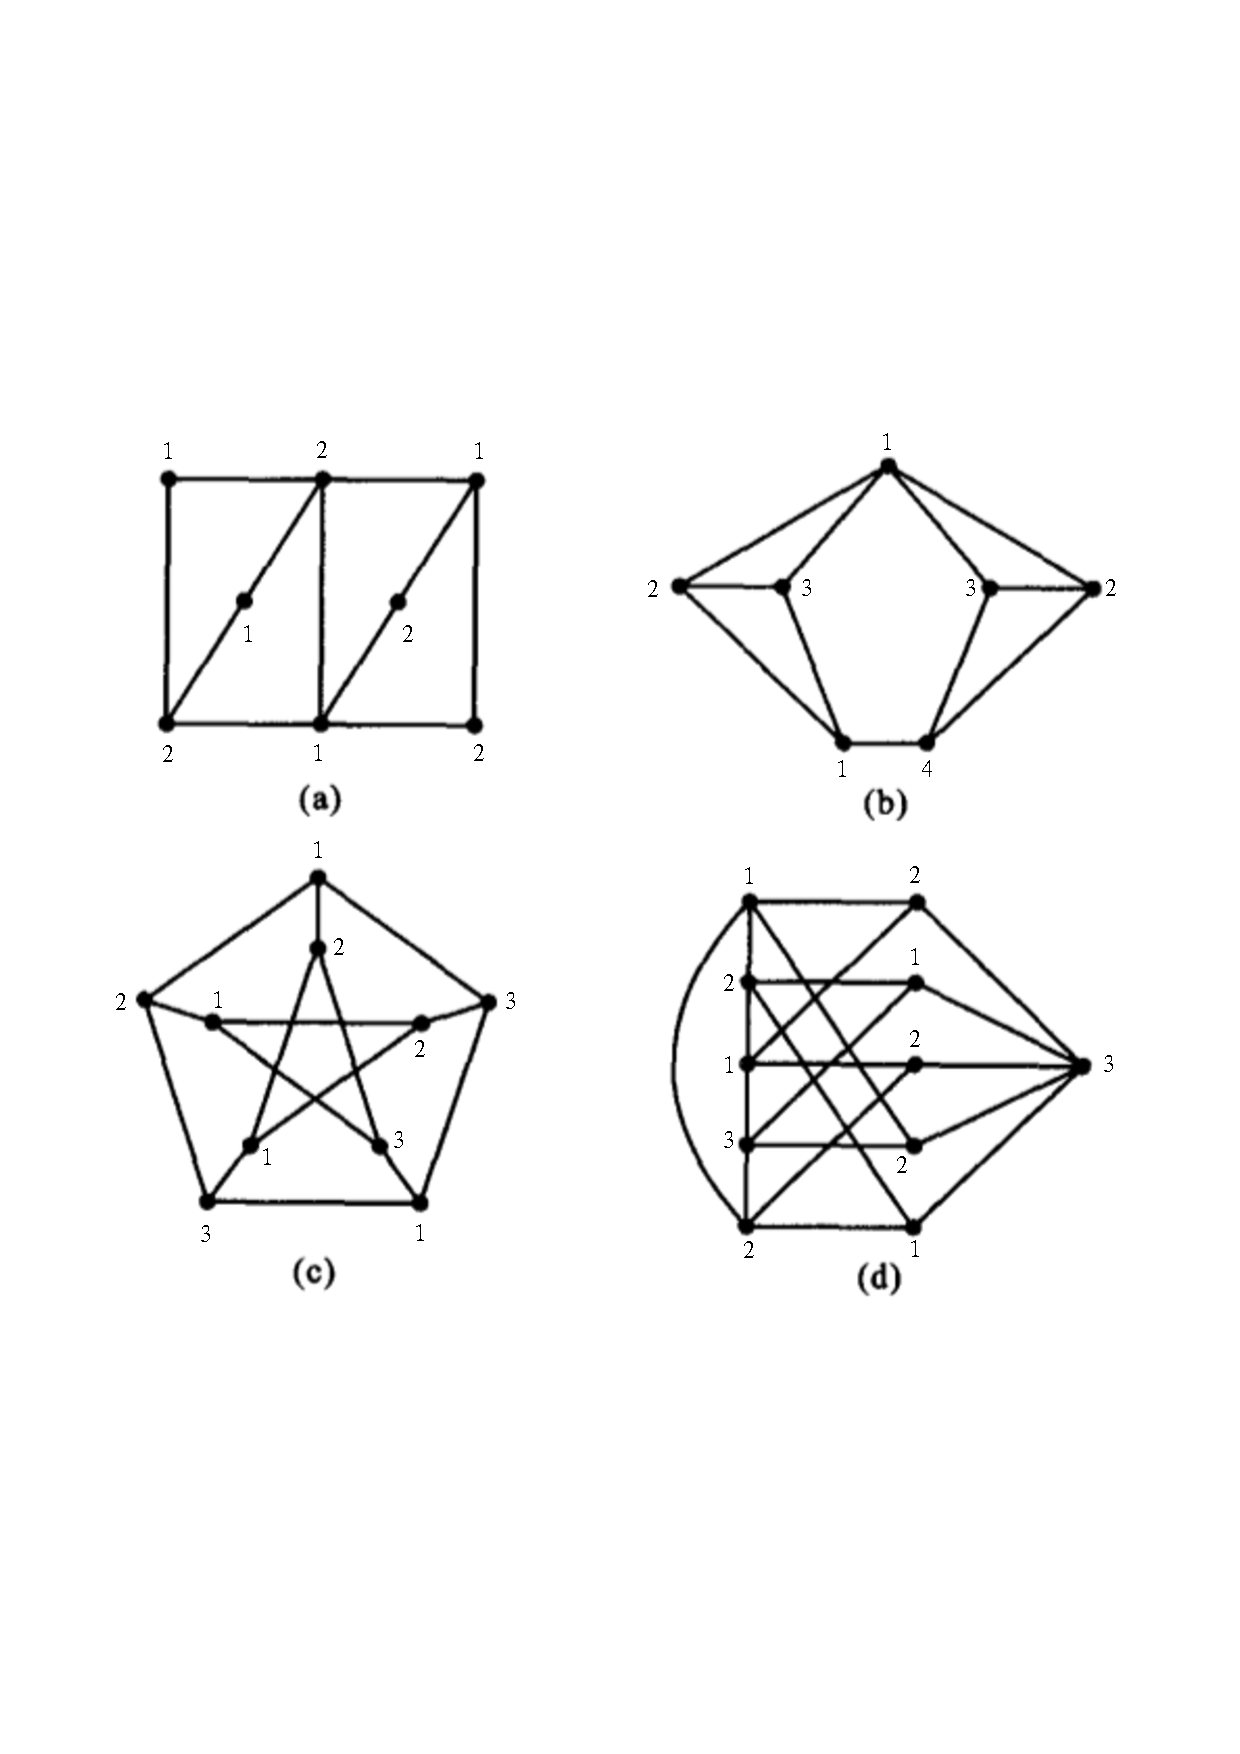
\includegraphics[scale=0.45]{image/ex7.1dot.pdf}
	\caption{}
	\label{fig:7.1dot}
\end{figure}
\end{proof}

\begin{example}
	证明: 若\(G\)是\(n\)阶非空的正则简单图且\(n\)为奇数,则\(\chi^{\prime}=\Delta+1\).
\end{example}

\begin{proof}
	由于图\(G\)是奇数阶图,故设图\(G\)的点数为\(n=2k+1,k\in\bbN^+\),边数为\(m\). 且图\(G\)是非空正则图,因此图\(G\)任意一点的度数均为\(\Delta\). 根据握手定理可知
	\begin{align*}
		2m&=\sum_{v\in V(G)}d(v)=n\Delta\\
		&=(2k+1)\Delta\\
		&>2k\Delta,
	\end{align*}
	即\(m>k\Delta\). 故\(\chi^{\prime}=\Delta+1\).
\end{proof}

\begin{example}
	证明: 每个\(3\)正则Hamilton图都有Tait着色.(\(3\)正则图的正常\(3\)边着色称为Tait着色)
\end{example}

\begin{proof}
	设图\(G\)是\(3\)正则的Hamilton图,\(C\)是图\(G\)的一个Hamilton圈,则\(C\)是偶圈,即\(C\)是\(2\)可正常边着色的. 且\(G-C\)是图\(G\)的一个\(1\)因子,即\(G-C\)是\(1\)可正常着色的. 故图\(G\)是\(3\)可正常边着色的,即图\(G\)可Tait着色.
\end{proof}

\begin{example}\label{ex:28}
	计算图\ref{fig:7.28}中各图的色多项式:
	\begin{figure}[H]
		\centering
		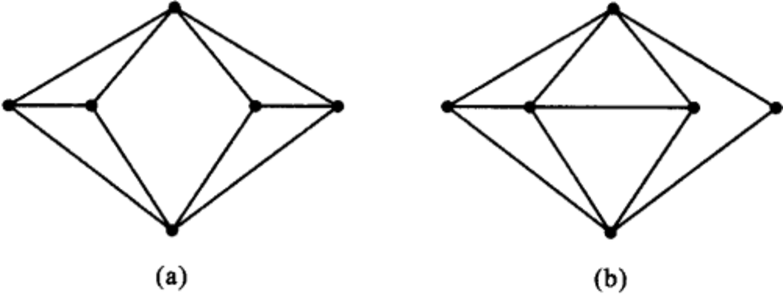
\includegraphics[scale=0.60]{image/ex7.28.pdf}
		\caption{}
		\label{fig:7.28}
	\end{figure}
\end{example}

\begin{proof}
	\begin{enumerate}[(a)]
		\item 图\ref{fig:7.28}中(a)的补图\(\bar{G}_a\)为
		\begin{figure}[H]
			\centering
			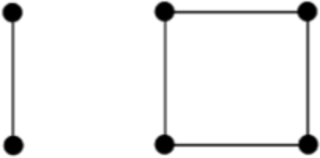
\includegraphics[scale=0.65]{image/ex7.28a.pdf}
			\caption{}
			\label{fig:7.28a}
		\end{figure}
		\(\bar{G}_a\)的两个连通分支分别记为\(\bar{G}_a^1\)和\(\bar{G}_a^2\).

		\(\bar{G}_a^1\)的伴随多项式为\(h(\bar{G}_a^1,x)=x+x^2\);

		设\(\bar{G}_a^2\)的伴随多项式为
		\[h(\bar{G}_a^2,x)=r_1x+r_2x^2+r_3x^3+r_4x^4,\]
		由于\(N_1(\bar{G}_a^2)=0,N_2(\bar{G}_a^2)=2,N_3(\bar{G}_a^2)=4,N_4(\bar{G}_a^2)=1\),故\(\bar{G}_a^2\)的伴随多项式为
		\[h(\bar{G}_a^2,x)=2x^2+4x^3+x^4.\]
		因此\(\bar{G}_a\)的伴随多项式为
		\begin{align*}
			h(\bar{G}_a,x)&=h(\bar{G}_a^1,x)\cdot h(\bar{G}_a^2,x)\\
			&=(x+x^2)\cdot(2x^2+4x^3+x^4)\\
			&=2x^3+6x^4+5x^5+x^6.
		\end{align*}
		故\(G_a\)的色多项式为
		\[P_k(G_a)=2[k]_3+6[k]_4+5[k]_5+[k]_6,\]
		其中\([k]_i=k(k-1)\cdots(k-i+1)\). 即
		\[P_k(G_a)=k(k-1)(k-2)^2(k^2-5k+8).\]
		\item 图\ref{fig:7.28}中(b)的补图\(\bar{G}_b\)为
		\begin{figure}[H]
			\centering
			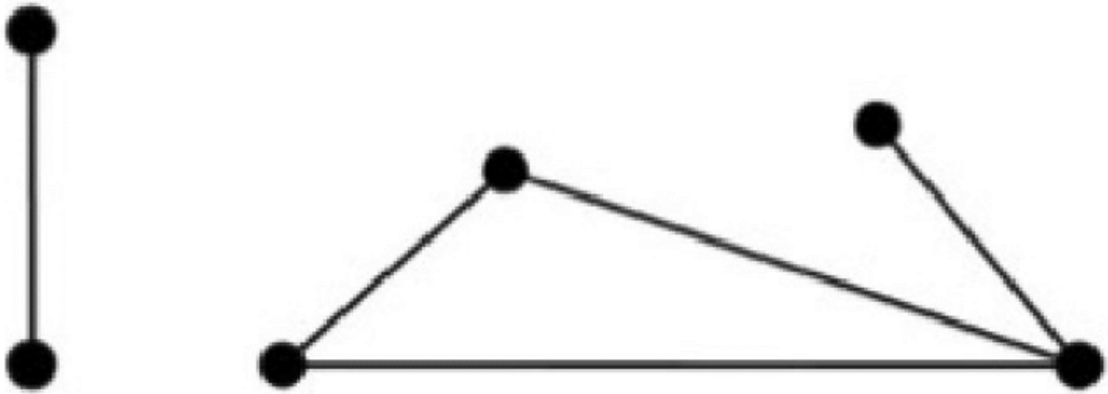
\includegraphics[scale=0.265]{image/ex7.28b.pdf}
			\caption{}
			\label{fig:4.1}
		\end{figure}
		\(\bar{G}_b\)的两个连通分支分别记为\(\bar{G}_b^1\)和\(\bar{G}_b^2\).

		\(\bar{G}_b^1\)的伴随多项式为\(h(\bar{G}_b^1,x)=x+x^2\);

		设\(\bar{G}_b^2\)的伴随多项式为
		\[h(\bar{G}_b^2,x)=r_1x+r_2x^2+r_3x^3+r_4x^4,\]
		由于\(N_1(\bar{G}_b^2)=0,N_2(\bar{G}_b^2)=2,N_3(\bar{G}_b^2)=4,N_4(\bar{G}_b^2)=1\),故\(\bar{G}_b^2\)的伴随多项式为
		\[h(\bar{G}_b^2,x)=2x^2+4x^3+x^4.\]
		因此\(\bar{G}_b\)的伴随多项式为
		\begin{align*}
			h(\bar{G}_b,x)&=h(\bar{G}_b^1,x)\cdot h(\bar{G}_b^2,x)\\
			&=(x+x^2)\cdot(2x^2+4x^3+x^4)\\
			&=2x^3+6x^4+5x^5+x^6.
		\end{align*}
		故图(b)与图(a)具有相同的色多项式,即
		\[P_k(G_b)=k(k-1)(k-2)^2(k^2-5k+8).\]
	\end{enumerate}
\end{proof}

\begin{example}
	试证图\ref{fig:7.32}所示的两个不同构的图\(G_1\)与\(G_2\)有相同的色多项式.
	\begin{figure}[H]
		\centering
		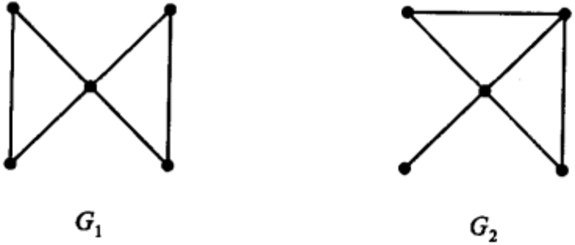
\includegraphics[scale=0.55]{image/ex7.32.pdf}
		\caption{}
		\label{fig:7.32}
	\end{figure}
\end{example}

\begin{proof}
	图\ref{fig:7.32}中\(G_1\)和\(G_2\)的补图分别如图\ref{fig:7.32_bt}所示
	\begin{figure}[H]
		\centering
		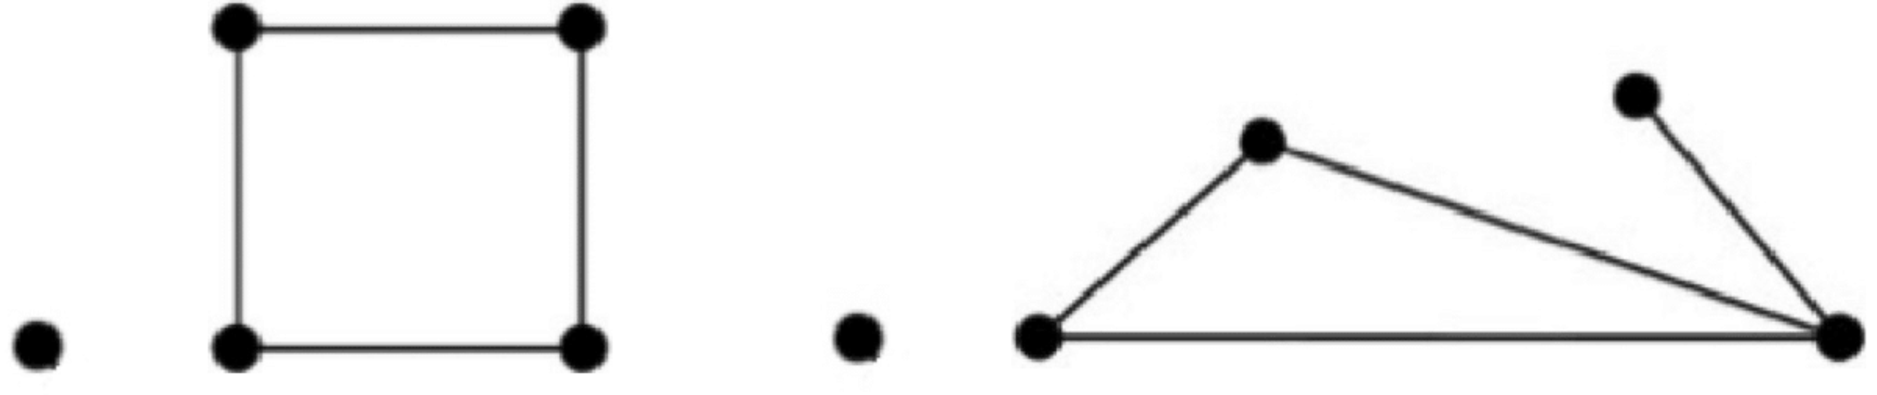
\includegraphics[scale=0.25]{image/ex7.32_bt.pdf}
		\caption{}
		\label{fig:7.32_bt}
	\end{figure}
	结合习题\ref{ex:28}的结论可知
	\begin{align*}
		h(\bar{G}_1,x)=h(\bar{G}_2,x)&=x(2x^2+4x^3+x^4)\\
		&=2x^3+4x^4+x^5.
	\end{align*}
	因此图\(G_1\)和\(G_2\)具有相同的伴随多项式. 故图\(G_1\)和\(G_2\)有相同的色多项式,即
	\begin{align*}
		P_k(G_1)=P_k(G_2)=&\text{ }2[k]_3+4[k]_4+[k]_5\\
		=&\text{ }2k(k-1)(k-2)+4k(k-1)(k-2)(k-3)\\
		&\text{ }+k(k-1)(k-2)(k-3)(k-4)\\
		=&\text{ }k(k-1)^2(k-2)^2.
	\end{align*}
\end{proof}

\end{document}
